% \begin{tikzpicture}[scale=0.5]
% \begin{scope}	
%     \begin{axis}[
% 		y=4cm,
% 		x=1cm,
% 		 clip=false,
% 		 xmin=-10,xmax=10,
% 		 xlabel= $\omega$,
% 		 ylabel={$X(j\omega)$},
% 		 ymin=-0.5,ymax=1.2,
% 		 axis lines=middle,
%          	%xtick={-5, -4, ..., 5},
% 		 %ytick={-1, 1},
% 		 yticklabels=\empty,
% 		 xticklabels=\empty,
% 		 every axis x label/.style={at={(ticklabel* cs:1.05)}, anchor=west,},
% 		every axis y label/.style={at={(ticklabel* cs:1.05)}, anchor=south,},
%      ]
% 		%\addplot+[red, smooth, mark=none] table [x={n}, y={xn}] {periodic_square_fs_samples_of_envilope_gen.dat};
% 		\addplot [red, dashed, domain=-10:10, samples=200] plot{2*sin(deg(x)*2*pi/8*2)/(pi*x)};
% 		\addplot [thick, blue, ->, ycomb, domain=-10:10] plot{2*sin(deg(x)*2*pi/8*2)/(pi*x)};
% 		\node at (axis cs:0, 1) [anchor=east] { $\pi$ };
% 		\draw[latex-] (axis cs:pi/3, 0) --(axis cs:0.6,-0.3) node  [anchor=north] { $\pi/W$ } ;
% 		\draw[latex-] (axis cs:-pi/3, 0) --(axis cs:-0.6,-0.3) node  [anchor=north] { $-\pi/W$ } ;		
%     \end{axis}
% \end{scope}	
% \end{tikzpicture} 

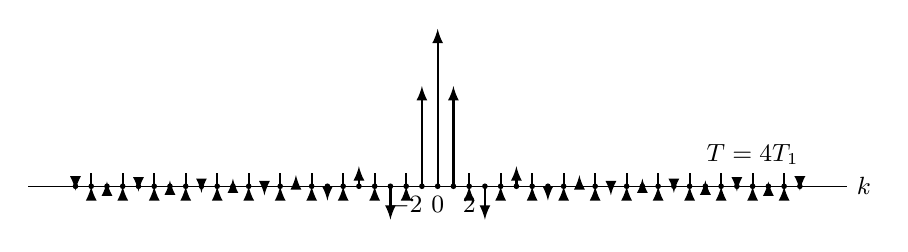
\begin{tikzpicture}[scale=0.4]
	\def\w{{-23,-22,-21,-20,-19,-18,-17,-16,-15,-14,-13,-12,-11,-10,-9,-8,-7,-6,-5,-4,-3,-2,-1,0,1,2,3,4,5,6,7,8,9,10,11,12,13,14,15,16,17,18,19,20,21,22,23}}
	\def\akmag{{-0.013840,0.000000,0.015158,-0.000000,-0.016753,0.000000,0.018724,-0.000000,-0.021221,0.000000,0.024485,-0.000000,-0.028937,0.000000,0.035368,-0.000000,-0.045473,0.000000,0.063662,-0.000000,-0.106103,0.000000,0.318310,0.500000,0.318310,0.000000,-0.106103,-0.000000,0.063662,0.000000,-0.045473,-0.000000,0.035368,0.000000,-0.028937,-0.000000,0.024485,0.000000,-0.021221,-0.000000,0.018724,0.000000,-0.016753,-0.000000,0.015158,0.000000,-0.013840}}


	\begin{scope}	
		\draw (-13, 0) -- (13,0) node[anchor=west] {\small $k$};
		\foreach \k in {-2, 0, 2}
		{
			\node at (\k/2, 0) [anchor=north] {\small $\k$};
		}
		%\node at (0,5) [anchor=south] {\small $Ta_k$};
		
		\foreach \k in {0,1, ..., 46}
		{
			\pgfmathparse{\w[\k]/2}
			\edef\wk{\pgfmathresult}
			\pgfmathparse{\akmag[\k]}
			\edef\akmagk{\pgfmathresult}	
			\draw[thick, -latex] (\wk, 0) -- ++(0,10*\akmagk);% node [anchor=south] {\small $\akmagk$};
			\ifthenelse{\lengthtest{0 pt = \akmagk pt}}{\draw[fill=black]  (\wk,0) circle (2pt);}{}
		}
			\node at (10, 1) {\small $T= 4T_1$};		
	\end{scope}
	\end{tikzpicture}